% Generated by paper/build_imt_parameter_figures.py; do not hand edit.
% Q1 grid SHA-256: 1a48a6f4d5a4c6c1449f35cd7e5584b7a14d4a08f8effc2c4508497e8ef20058
\begin{figure}[!hbp]
\centering
\begin{minipage}[t]{\linewidth}
\centering
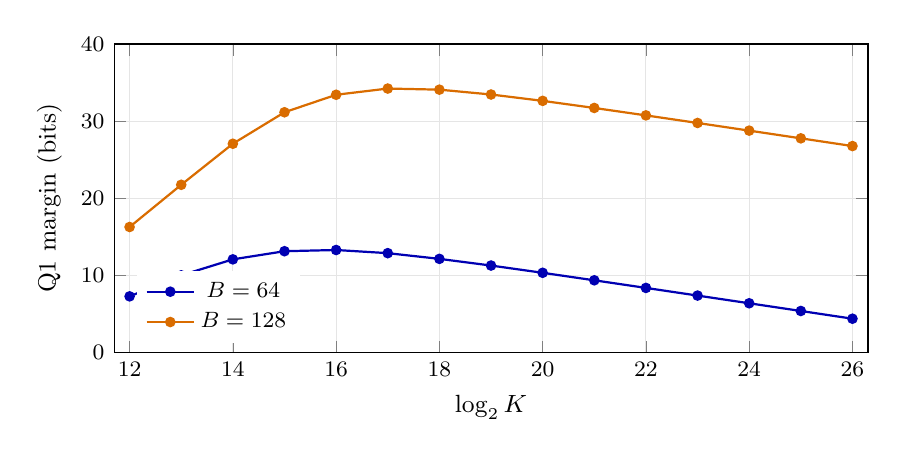
\begin{tikzpicture}
\begin{axis}[tick label style={font=\footnotesize},label style={font=\small},title style={font=\small},grid=major,grid style={black!10},legend style={font=\footnotesize,draw=none},width=.92\linewidth,height=5.5cm,xlabel={$\log_2 K$},ylabel={Q1 margin (bits)},xmin=11.7,xmax=26.3,ymin=0,ymax=40,xtick={12,14,16,18,20,22,24,26},legend pos=south west,]
\addplot[blue!70!black,thick,mark=*,mark size=1.5pt] coordinates {(12,7.2854857489) (13,10.0090201085) (14,12.0832614441) (15,13.1390922468) (16,13.2963998191) (17,12.8871610268) (18,12.1466382431) (19,11.2810369722) (20,10.3403771086) (21,9.3679471183) (22,8.3815223483) (23,7.3876553599) (24,6.3899560564) (25,5.3901051543) (26,4.3889026631)};
\addlegendentry{$B=64$}
\addplot[orange!85!black,thick,mark=*,mark size=1.5pt] coordinates {(12,16.2784460297) (13,21.7503698500) (14,27.0735386208) (15,31.1534629535) (16,33.4221485975) (17,34.2276637311) (18,34.0849090219) (19,33.4552570471) (20,32.6317852093) (21,31.7117191602) (22,30.7488362012) (23,29.7657818858) (24,28.7725947112) (25,27.7739122608) (26,26.7719414261)};
\addlegendentry{$B=128$}
\end{axis}
\end{tikzpicture}
\end{minipage}
\caption{IMT one-active-row bounds versus message length, with $(t,s)=(64,20)$.
The two outers share the same maps. These binary64 Q1 evaluations do not
include higher occupancies. Markers are evaluated configurations;
connecting segments are visual guides in all three parameter-slice figures.}
\label{fig:finite-k-b}
\end{figure}
